\section{Simulation}
\rhead{Simulation}

Der erste Schritt ist ein Modell zu erstellen.
Dazu wird der Golfstrom in drei Zonen aufgeteilt. Die jeweiligen Polarregionen und der Äquator werden je zu eine Zone. Diese Zonen erhalten dann je eine Box.
Im laufe des Seminars wurden zwei Modelle erstellt. Der erste Ansatz war sehr lehrreich hatte aber  schlussendlich nichts mit dem realen Golfstrom gemeinsam. Der zweite Ansatz war erfolgreicher und der Golfstrom kann mit diesem Modell qualitativ simuliert werden.
In den folgenden zwei Kapiteln werden diese zwei Modelle vorgestellt und die jeweiligen Resultate diskutiert.

\subsection{Zwei-Fluss Modell(1.Ansatz)}

In diesem Modell werden die Boxen jeweils durch Rohre verbunden wie im 2-Box Modell. Nun werden jedoch zwei flüsse simuliert, die von den jeweiligen Dichtegradienten der Unterschiedlichen Boxen abhängen. $q_1$ ist also nur vom Dichteunterschied zwischen Box $1$ und Box $2$ abhängig. Dementsprechend hängt auch $q_2$ nur vom Dichteunterschied der Boxen $2$ und $3$ ab.
Der Vorteil der Aufteilung der Flüsse ist, dass wir sie entkoppeln können und sie nicht von der jeweiligen dritten Box abhängig sind.
Eine Darstellung des Modelles ist in Abbildung 9.4 zu finden.

\begin{figure}
	\centering
	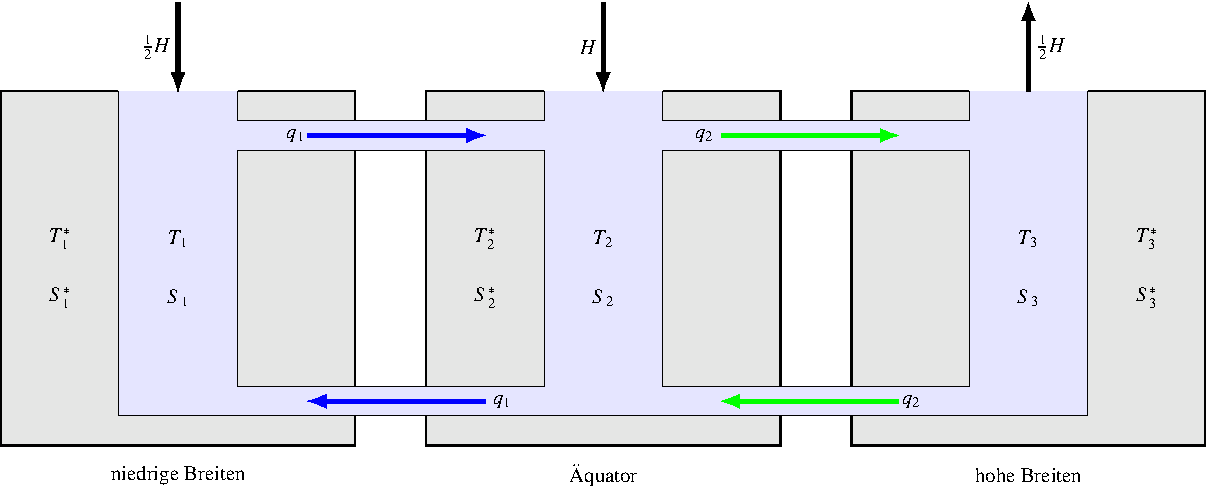
\includegraphics[width=14cm]{thermohalin/tikz/3b2f.pdf}
	\caption{Zwei-Fluss Modell des THC}
		\label{thermohalin:3b2f}
\end{figure}

So lassen sich nun für jede Box die zugehörigen Salinitäts- und Temperaturgleichungen aufstellen. So ist auch ersichtlich, dass Box $1$ und $3$ jeweils einen Fluss in der Gleichung haben. Im Gegensatz dazu hat Box $2$ jedoch zwei Flüsse in der Gleichung. Das liegt daran, dass wie aus der Abbildung ersichtlich, die mittlere Box von beiden Strömen durchflossen wird.


\begin{equation}
\begin{aligned}
\frac{dT_1}{dt} &= c(T_1^*-T_1)&+|q_1|(T_2-T_1)\phantom{+|q_2|(T_3-T_2)}
\\
\frac{dT_2}{dt} &= c(T_2^*-T_2)&+|q_1|(T_1-T_2)+|q_2|(T_3-T_2)
\\
\frac{dT_3}{dt} &= c(T_3^*-T_3)&+ \phantom{+|q_1|(T_1-T_2)}|q_2|(T_2-T_3)
\end{aligned}
\end{equation}
\begin{equation}
\begin{aligned}
\frac{dS_1}{dt} &= -H/2 &+ d(S_1^*-S_1)&+|q_1|(S_2-S_1)\phantom{+|q_2|(S_3-S_2)}
\\
\frac{dS_2}{dt} &= \phantom{-}H &+ d(S_2^*-S_2)&+|q_1|(S_1-S_2)+|q_2|(S_3-S_2)	
\\
\frac{dS_3}{dt} &= -H/2 &+d(S_3^*-S_3)&+ \phantom{+|q_1|(S_1-S_2)}|q_2|(S_2-S_3)
\end{aligned}
\end{equation}	

Dazu die Flussgleichungen die jeweils nur von den Dichteunterschied der jeweiligen Boxen abhängig sind:

\begin{equation}
\begin{aligned}
 q1 &= k[\alpha(T_2-T_1)-\beta(S_2-S_1)] 
 \\
 q2 &= k[\alpha(T_3-T_2)-\beta(S_3-S_2)]
\end{aligned}
\end{equation}

\subsubsection{Matlab-Code der Simulation}

Als Ziel ist es, die oben aufgestellten Differentialgleichungen mittels Matlab zu lösen. Dies wird mit dem Differentialgleichungslöser ode45 aus der Matlab Funktionenbibliothek erreicht.
Dazu müssen wir der Funktion nur einen Zustandsvektor, einen Zeitvektor und die Konstanten der jeweiligen Umgebungstemperaturen und Salinitäten übergeben.
\lstinputlisting[style=Matlab]{thermohalin/listings/input.m} 
Diese werden wie folgt dem Differentialgleichungslöser übergeben:
\lstinputlisting[style=Matlab]{thermohalin/listings/listing-ode45.m} 

Daraufhin wird im File \texttt{odefun-3Box.m} Das Gleichungssystem schrittweise gelöst und die Resultate zurückgegeben. Gleichzeitig wird der Zustandsvektor mit $0$ initialisiert und die Naturkonstanten zur Flussberechnung definiert.

\lstinputlisting[style=Matlab]{thermohalin/listings/listing-solve.m}

Die Rückgabewerte werden in einem Array gespeichert und dann geplottet. Um den Text nicht in die Länge zu ziehen wird hier nur das der code zur erstellung des Temperaturplots dargestellt. Die Salinität folgt dem gleichen Schema.
Da die Flüsse innerhalb der ode45-Funktion berechnet wurden, muss dies nachträglich noch einmal gemacht werden, da die Werte ja geplottet werden. Dazu müssen die jeweiligen Werte aus dem Lösungsvektor extrahiert und die Flüsse wiederholt berechnet werden.
\lstinputlisting[style=Matlab]{thermohalin/listings/listing-plot.m}

Die So entstehenden Figuren werden im Folgenden Kapitel ausgewertet und Diskutiert. 

\subsubsection{Resultate}


Soweit sieht alles vielversprechend aus und die ersten Durchläufe ergaben auch brauchbare Resultate. Wenn nun jedoch mit den Umgebungsvariablen gespielt wird treten plötzlich unmögliche Phänomene auf.
Einer der beiden Flüsse ist negativ und ändert seine Richtung. Das resultiert in zwei gegenläufigen Strömen welche in keiner Weise mit dem Golfstrom übereinstimmen. Das führt dazu, dass am Äquator eine Absinkstelle entsteht. Sonst kann dieses Ereignis gar nicht eintreten. In der Realität ist klar zu erkennen, dass Absink- und Aufsteigstellen jeweils nur an den Polen vorhanden sind. 
Ein Plot der Simulationsresultate findet sich in Abbildung \ref{thermohalin:simulationsresultate}.

\begin{figure}
	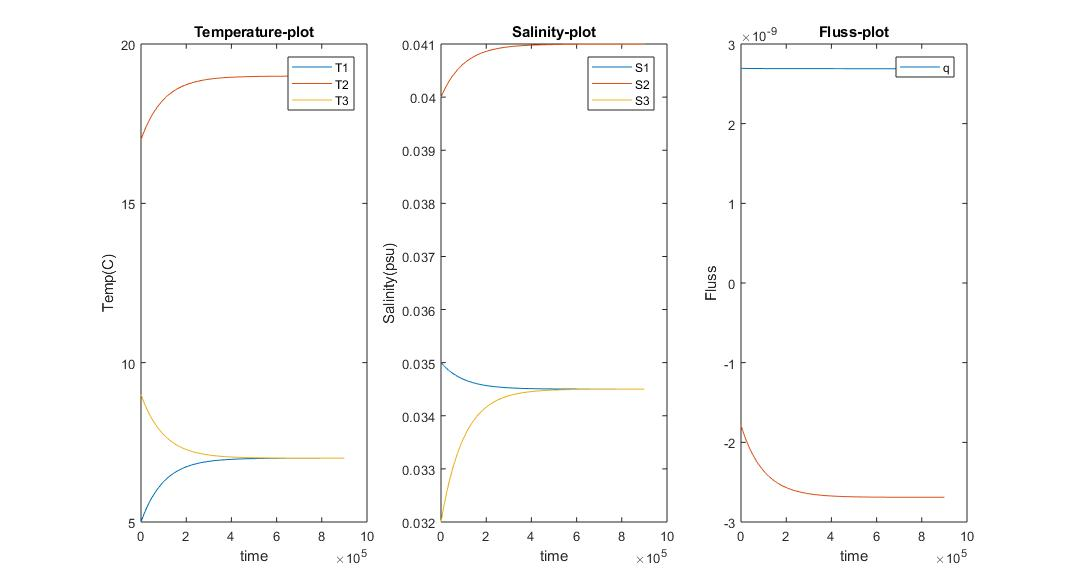
\includegraphics[width=14cm]{thermohalin/Code/graphs/result-3b2f-script.jpg}
	\centering
	\caption{Simulationsresultate}
	\label{thermohalin:simulationsresultate}
\end{figure}

Durch die Entkoppelung der zwei Flüsse, war es möglich, dass ein Fluss seine Richtung ändert.
Simulationstechnisch gesehen, hat das Modell funktioniert. Nur ist das Modell Fehlerhaft. Das Modell muss also angepasst werden. Das Resultat Der Anpassung ist in Abbildung \ref{thermohalin:3b2f-inverted} zu sehen.

\begin{figure}
	\centering
	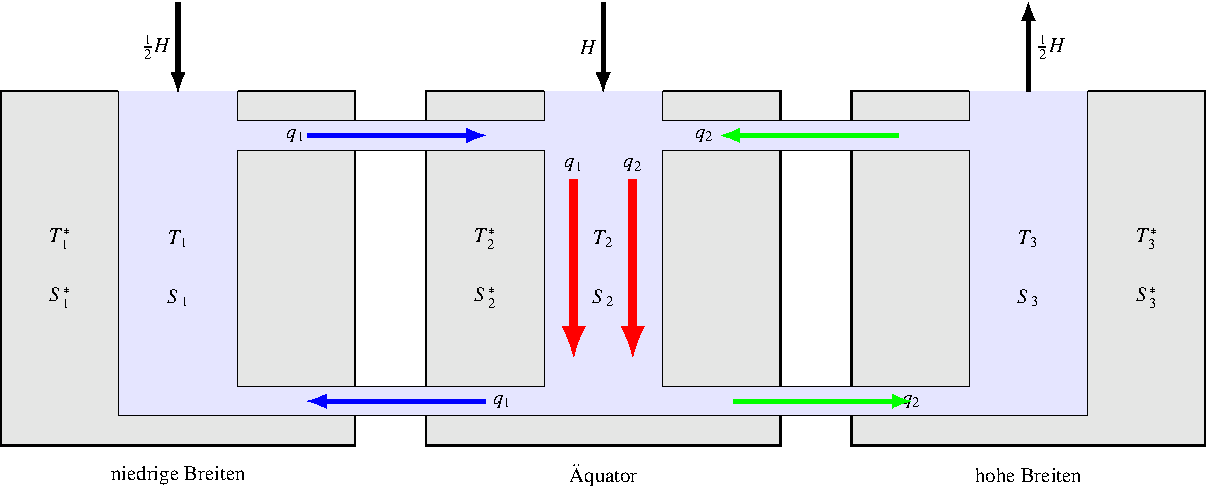
\includegraphics[width=14cm]{thermohalin/tikz/3b2f-inverted.pdf}
	\caption{Angepasstes Zwei-Fluss Modell}
	\label{thermohalin:3b2f-inverted}
\end{figure}

Nun lässt sich die neu entstandene Absinkstelle auch sofort erkennen. 
Mit diesem Modell lässt sich der Golfstrom also nicht erfolgreich simulieren. 
Der nächste, erfolgreichere, Ansatz wird im nächsten Unterkapitel vorgestellt.

\subsection{Ein-Fluss Modell} 

Dieses Modell ist der verbesserte Nachfolger des Zwei-Fluss Modelles.
Es stammt aus einer Aufgabe des Seminarbuches \texttt{Mathematics and Climate} \cite{skript:kaperengler}.

Um zu verhindern, dass in der mittleren Box eine zusätzliche Absinkzone entsteht, muss dieser Weg versperrt werden. Das erreicht man am einfachsten, wenn der Tiefenstrom von der Äquatorbox getrennt wird. Die Äquatorzone ist so nur via Oberflächenströmungen mit den anderen Boxen verbunden und die Tiefenströmung verbindet nur die Polzonen.


\begin{figure}
	\centering
	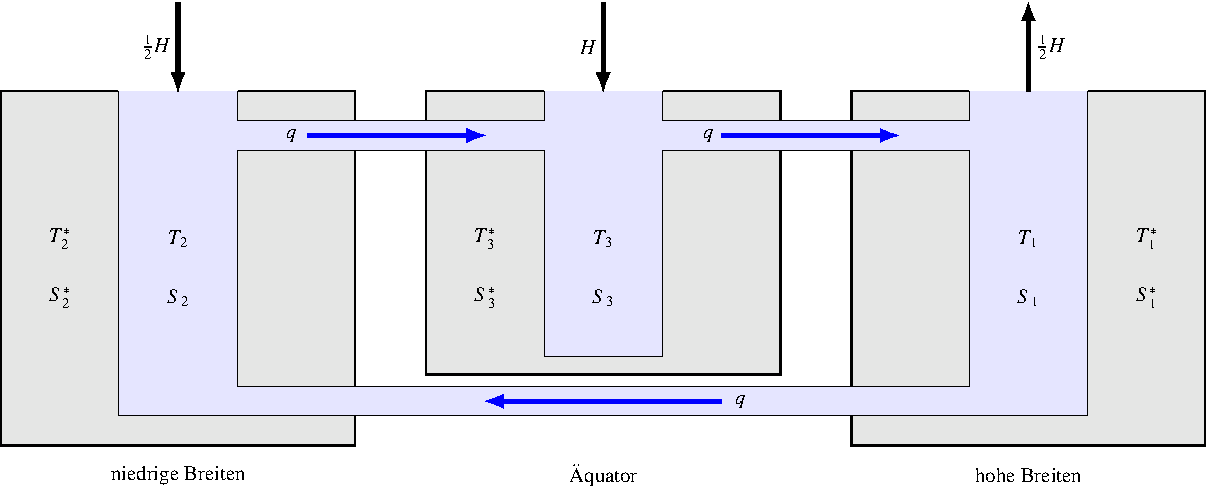
\includegraphics[width=14cm]{thermohalin/tikz/3b1f.pdf}
	\caption{Ein-Fluss Modell des THC}
	\label{thermohalin:3b1f}
\end{figure}

Aus diesem Modell lassen sich nun neue Gleichungen für die Boxen aufstellen:

\begin{equation}
\begin{aligned}
\frac{dT_1}{dt} &= c(T_p-T_1)&+ \begin{cases} q(T_3-T_1) & \quad q>0 \\ |q|(T_2-T_1) & \quad q<0 \end{cases}
\\
\frac{dT_2}{dt} &= c(T_p-T_2)&+\begin{cases} q(T_1-T_2) & \quad q>0 \\ |q|(T_3-T_2) & \quad q<0 \end{cases}
\\
\frac{dT_3}{dt} &= c(T_e-T_3)&+\begin{cases} q(T_2-T_3) & \quad q>0 \\ |q|(T_1-T_3) & \quad q<0 \end{cases}
\end{aligned}
\end{equation}
\begin{equation}
\begin{aligned}
\frac{dS_1}{dt} &= -H/2 &+ d(S_p-S_1)&+\begin{cases} q(S_3-S_1) & \quad q>0 \\ |q|(S_2-S_1) & \quad q<0 \end{cases}
\\
\frac{dS_2}{dt} &= \phantom{-}H &+ d(S_p-S_2)&+\begin{cases} q(S_1-S_2) & \quad q>0 \\ |q|(S_3-S_2) & \quad q<0 \end{cases}	
\\
\frac{dS_3}{dt} &= -H/2 &+d(S_e-S_3)&+\begin{cases} q(S_2-S_3) & \quad q>0 \\ |q|(S_1-S_3) & \quad q<0 \end{cases}
\end{aligned}
\end{equation}	
\subsubsection{Matlab-code}

Erklärung der Änderung, (Codeausschnitte)


\subsubsection{Resultate} 

1. Resultat normale Simulation mit aktuellen Werten

2. Simulation der werte nach klimaerwärmung

3. Vergleich Paper Liu Wei


